\documentclass{article}
\title{Math 425 Assignment 2}
\author{Max Horowitz-Gelb, Tushar Verma}
\date{October 30, 2016}
\usepackage{graphicx}
\usepackage{amsmath}
\DeclareMathOperator*{\argmin}{argmin}

\setlength{\parindent}{0pt}
\setlength{\parskip}{10pt}

\begin{document}
\maketitle
\section*{Problem 1}
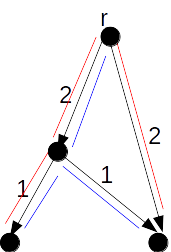
\includegraphics[scale=0.5]{tree}

In this figure the minimum spanning tree is labeled with blue lines and the tree created of least cost dipaths is labeled with red lines. These two trees are clearly different from eachother. As one can see the MST does not contain all least cost dipaths since the cost from $r$ to the bottom right node is of cost 3 and there is a cheaper path of cost 2. Conversely the cost of the tree made from the minimum cost dipaths is of cost 5 but the MST is of cost 4, therefore the minimum dipath tree is not an MST.
\section*{Problem 2}
Given a digraph $G = (V,E)$, costs $c_e$ for every $e \in E$ and disjoint sets $R,S \subset V$. Then the problem of finding a least cost dipath starting from any node in $R$ and ending in any node in $S$ can be reduced to solving one ordinary shortest path problem by lightly modifying $G$. Simply make a new graph by adding a special node $\gamma$ to $V$ and edges from $\gamma$ to all nodes in $R$, all with cost $0$. Call this new graph  $G'$.

If G has no negative cost dicircuits, then if we run ordinary least cost dipaths on $G'$ with $r = \gamma$ and achieve a feasible potential $y$ and least cost paths
described by 
$p$, our least cost dipath from $R$ to $S$ in $G$ is a dipath that ends in $t = \argmin\limits_{v \in S} y_v$. Its cost is $y_t$ and its path is described by $p(f)$ with node $\gamma$ and edge containing $\gamma$ removed.

First note that $G$ has no negative cost dicircuits if and only if $G'$ does not either since $\gamma$ has only outgoing edges and cannot introduce any new circuits.

We shall prove this is valid via contradiction. Assume that there exists a path from node $a \in R$ to $b \in S$ in $G$ with less cost than any path found from ordinary least cost dipaths on $G'$. Then $y_b$ would be greater than the cost of this path. But there there is a 0 cost edge from $\gamma$ to $a$ making $y_a = 0$ so if such a path existed then it would give a lower cost path from $\gamma$ to $b$. Since $G$ is a subgraph of $G'$ this creates a contradiction. 

Finally if $G$ had a negative cost dicircuit then so would $G'$ and running ordinary least cost dipaths on $G'$ would discover this. This would imply there is no solution to the problem.
 
\section*{Problem 3}
Suppose that we are give a shortest path problem on a digraph $G$ such that a node $w\neq r$ is incident with two arcs $a$ and $b$. Then we can answer the problem with a smaller digraph in three different ways. 

If $w$ has only outgoing arcs, then clearly there is no path from $r$ to $w$. 
Hence we can solve the shortest dipath problem on $G$ with $w$ removed and then simply set $y_w = \inf$ and $p(w) = -1$. 

If $w$ has only incoming arcs, then clearly there is no path from $r$ to $v$ where $v \neq w$ and $w$ is in said path. Then let $a = \alpha w$ and $b = \beta w$. Then we may again remove $w$ from $G$ and solve for the least cost dipaths to aquire $y$ and $p$. 
Then $y_w = min \{ y_\beta + c_b, y_\alpha + c_a\} $ and
$p(w) = v$ such that $(v,e) \in \{(\alpha,a), (\beta,b)\}$ and $y_w = y_v + c_e$.

If $w$ has one incoming arc and one outgoing arc, then we can combine those arcs into a single arc to solve a smaller problem. Let $a = \alpha w$ and let $b = w \beta$ and let $f$ be an arc from $\alpha$ to $\beta$ if it exists. Then there are 2 cases.

\subsection*{Case 1}
$f$ does not exist or $c_f > c_a + c_b$. 

If $f$ exists but the cost of going through $w$ rather than using $f$ is cheaper or if $f$ doesn't exist at all, then we can pretend like $f$ exists and its cost is that of going through $w$. This is because if it were cheaper to go through $w$ a shortest dipath would always choose that option over using $f$. And if $f$ didn't exist then pretending it exists can represent going through $w$. 

So what we do explicitly is ensure that $f$ exists and set its cost $c_f = c_a + c_b$. Then run ordinary least cost dipaths on the new graph. After getting back $y$ and $p$, if $p(\beta) = \alpha$ then set $p(\beta) = w$. If $y_\alpha \neq \inf$ then set $y_w = y_\alpha + c_a$ and set $p(w) = \alpha$.

Also if $w$ creates a negative dicircuit then this procedure would account for that since the smaller graph also would have to have a negative dicircuit.

\subsection*{Case 2}
$f$ does exist and $c_f < c_a + c+b$

By similar logic to case 1 here we would rather use $f$ than go through $w$. So we simply remove $w$ and run ordinary least cost dipaths on the resultant graph to aquire $y$ and $p$. Then if $y_\alpha \neq \inf$ then set $y_w = y_a + c_a$ and $p(w) = \alpha$. 

This similarly accounts for dicircuits. 

In both cases there are a constant number of operations so the reduction costs are $O(1)$. Therefore this whole procedure is the same time complexity as running ordinary least cost dipaths on a graph with $n-1$ nodes and $m-2$ edges. 


\end{document}

